\section{Experimental Results}
\ifCLASSOPTIONonecolumn\begin{figure*}[t]
\centering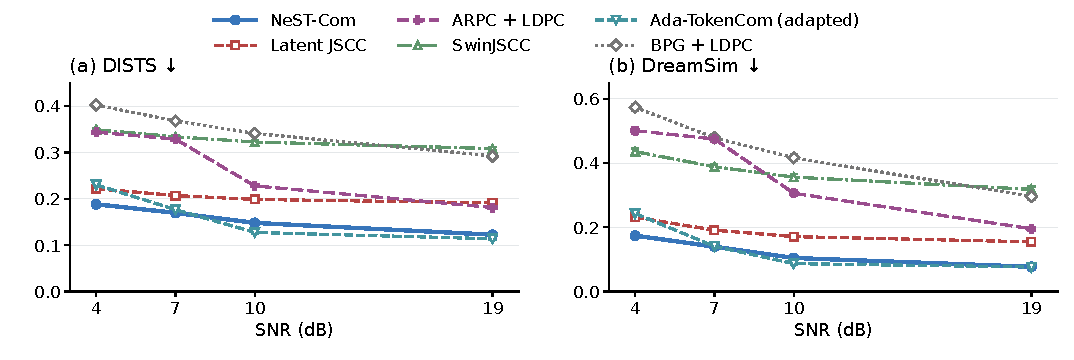
\includegraphics[width=\textwidth]{figure2.pdf}
\caption{Six-system reconstruction on common500 at $N=1024$. Points and bars are equal-source means and pointwise 95\% source-bootstrap intervals after averaging three channel realizations per source, including failures. Ada is the predicted-class, fixed-frame adaptation. Lower DISTS and DreamSim are favorable.}
\label{fig:performance}
\end{figure*}
\fi
\subsection{Experimental Setup}
The 500 ImageNet validation sources~\cite{imagenet} are disjoint from cal1000 and use fixed $256\times256$ preprocessing. We evaluate $N=1024$ at 4/7/10/19 dB and $N=512$ at 4/10/19 dB. Each point averages three channel realizations per source, retaining gray failures, before equal-source means and direct paired 95\% source-bootstrap intervals (10\,000 resamples). Controls use the first 100 full manifest IDs. Historical noise identities remain method/budget-specific; the matched-grid control shares noise.

Latent JSCC maps tokenizer latents to symbols with convolutional layers and shares $\Dc$, using MSE, LPIPS, and latent-consistency losses (100k updates). SwinJSCC~\cite{swinjscc} uses RGB MSE (200k updates, minimum calibration MSE selection). Both train on 20\,000 images for $256\times256$ and $N=1024$. Digital baselines include BPG~\cite{bpg} and ARPC~\cite{arpc} with LDPC/QAM. The predicted-class, fixed-frame Ada-TokenCom adaptation~\cite{adatokencom} retains LlamaGen-L/VQ16, prefix arithmetic coding, and sampled completion (CFG=4, $T=1$, top-$k=2000$, top-$p=1$). ConvNeXt predicts its transmitted 10-bit class; ARPC captions and all required fields are likewise paid. This comparison does not reproduce Ada's long-term budget controller or ARQ.

Decoder training and DINOv2 calibration are distinct from evaluation. DISTS~\cite{dists} and DreamSim~\cite{dreamsim} are the primary measures of source-referenced perceptual reconstruction. PSNR quantifies pixelwise fidelity; LPIPS-Alex~\cite{lpips} and CLIP-I~\cite{clip} are also reported. All metrics evaluate frozen systems on native float RGB. DISTS uses $256\times256$; DreamSim/CLIP use the frozen $224\times224$ bicubic-antialias preprocessing. Model, numerical-route and calibration details appear in Supplement~S1.

Processing uses 32 sources, two warmups and three measurements per source, batch one, one RTX PRO 6000 and two CPU cores. TX spans in-memory RGB to symbols; RX spans received symbols to RGB. Fresh probability evaluation, source coding, link processing and generation are included; loading, disk I/O and scoring are excluded. Original precision routes are retained; BPG is CPU-only on the same host/quota.

\begin{table}[t]
\caption{Within-scale transmission evidence. (A) NeST minus WHOLE under the frozen family policies. (B) Only endpoint granularity changes under matched model, MCS, ceiling, and noise. (C) Ordered receiver interventions on the actual NeST prefixes. Brackets are source-paired 95\% intervals; each block uses its stated population.}
\label{tab:internal}\centering\footnotesize
\setlength{\tabcolsep}{2.1pt}\renewcommand{\arraystretch}{1.05}
\begin{tabular}{@{}lccc@{}}\toprule
\multicolumn{4}{l}{\textit{A. common500, $N=1024$, family-specific policies}}\\
SNR & Util. W$\to$N (\%) & $\Delta$DISTS & $\Delta$DreamSim\\
\midrule
4 & 73.81$\to$99.56 & \shortstack{-0.0146\\{}[-0.0157, -0.0136]} & \shortstack{-0.0303\\{}[-0.0333, -0.0273]}\\[2pt]
7 & 83.19$\to$99.75 & \shortstack{-0.0060\\{}[-0.0097, -0.0021]} & \shortstack{-0.0108\\{}[-0.0157, -0.0057]}\\[2pt]
10 & 77.70$\to$99.79 & \shortstack{-0.0141\\{}[-0.0153, -0.0128]} & \shortstack{-0.0270\\{}[-0.0299, -0.0241]}\\[2pt]
19 & 85.24$\to$99.83 & \shortstack{-0.0048\\{}[-0.0053, -0.0043]} & \shortstack{-0.0043\\{}[-0.0051, -0.0036]}\\[2pt]
\midrule
\multicolumn{4}{l}{\textit{B. control100, 10 dB, common ceiling $(8,126)$}}\\
Grid (ends) & Utilization (\%) & DISTS & DreamSim\\
\midrule
Whole (5) & 78.13 & 0.1650 & 0.1387\\
Quarter (20) & 95.19 & 0.1535 & 0.1143\\
Eighth (39) & 97.44 & 0.1516 & 0.1137\\
Token (352) & 99.85 & 0.1505 & 0.1115\\
\midrule
\multicolumn{4}{l}{\textit{C. control100, 10 dB, same received prefixes}}\\
Intervention & $\Delta$PSNR (dB) & $\Delta$DISTS & $\Delta$DreamSim\\
\midrule
B0--A0 & \shortstack{+0.287\\{}[0.240, 0.335]} & \shortstack{-0.0062\\{}[-0.0077, -0.0048]} & \shortstack{-0.0113\\{}[-0.0147, -0.0083]}\\[2pt]
C0--B0 & \shortstack{+0.537\\{}[0.404, 0.682]} & \shortstack{-0.0083\\{}[-0.0102, -0.0065]} & \shortstack{-0.0159\\{}[-0.0205, -0.0116]}\\[2pt]
\bottomrule\end{tabular}\end{table}

\ifCLASSOPTIONonecolumn\else\begin{figure*}[t]
\centering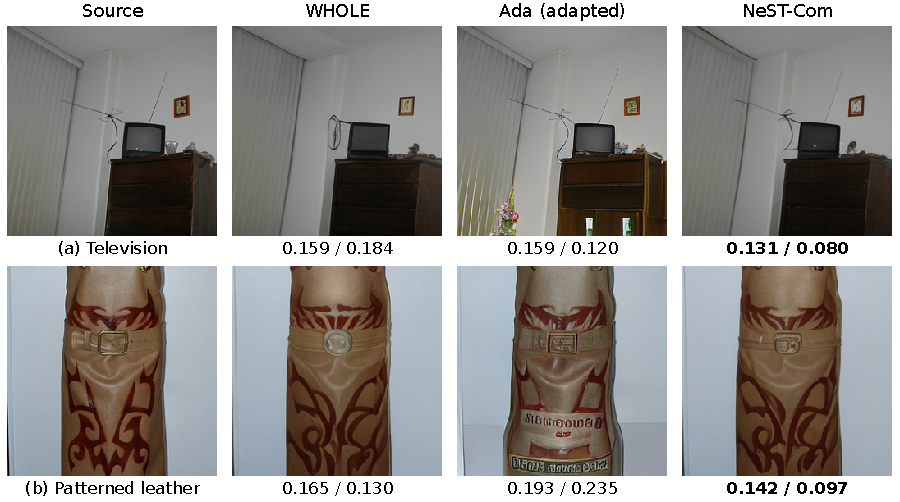
\includegraphics[width=6.0in]{figure3.pdf}
\caption{Selected qualitative comparisons at $N=1024$ and 7 dB. Columns show the source, WHOLE, fixed-frame Ada, and NeST-Com. Values are full-image DISTS$\downarrow$ / DreamSim$\downarrow$. Each output uses its method's fixed first channel realization; source identities and the selection protocol are in Supplement~S6.}
\label{fig:qualitative}
\end{figure*}
\fi
\subsection{Effect of Token-Wise Frame Fitting}
Table~\ref{tab:internal}(A) compares NeST-Com with WHOLE using shared tokenizer, prior, coder and receiver under frozen family policies. Across seven budget/SNR settings, all five metrics favor NeST in the source-paired intervals, improving both pixelwise fidelity and perceptual similarity. At $N=1024$, 10 dB, source-bit utilization rises from 77.70\% to 99.79\%, DISTS falls from 0.1621 to 0.1481, and DreamSim from 0.1317 to 0.1048. PSNR gains range from 0.45 to 0.88 dB over the four $N=1024$ points.

Block B isolates granularity on 100 sources with fixed model, 16-QAM rate 2/3, maximum position $(8,126)$ and shared noise. Whole/Quarter/Eighth/Token utilization is 78.13/95.19/97.44/99.85\%. Token--Quarter improves PSNR by $0.172\,[0.125,0.221]$ dB, with DISTS and DreamSim differences $-0.0030\,[-0.0041,-0.0020]$ and $-0.0028\,[-0.0050,-0.0006]$. Thus finer legal endpoints convert unused capacity into better reconstruction. Block A uses family-specific frozen policies.

Block C uses the same actual NeST prefixes for successive interventions. A0 retains prior completion; B0 adds the received boundary residual while retaining A0's future conditioning; C0 also updates that conditioning. At 10 dB, B0--A0 improves PSNR by 0.287 dB and reduces DreamSim by 0.0113. C0--B0 adds 0.537 dB and a 0.0159 reduction, respectively. Both stages have favorable paired intervals for these metrics and DISTS. Boundary information therefore contributes through both residual correction and subsequent prediction. Supplement~S3 reports 7 dB and the final-scale case, where no finer-scale propagation remains.

\subsection{Reconstruction Quality and Processing Cost}
\ifCLASSOPTIONonecolumn\begin{figure*}[t]
\centering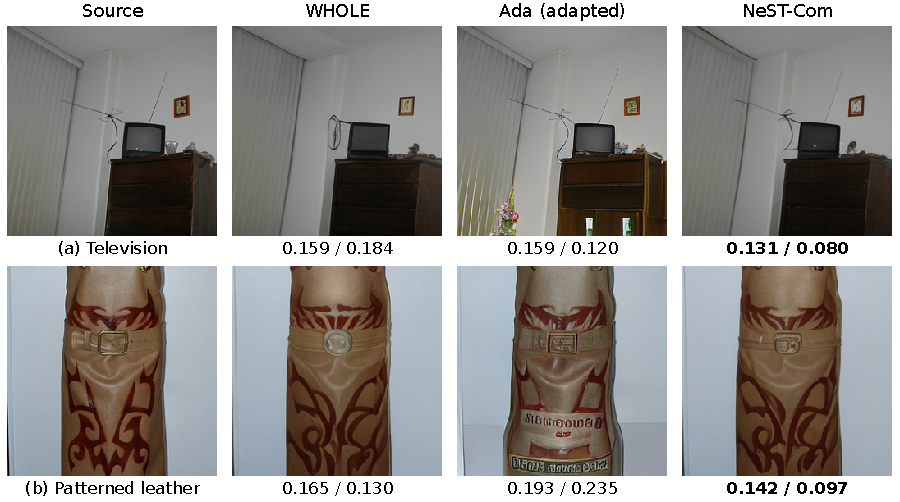
\includegraphics[width=6.0in]{figure3.pdf}
\caption{Selected qualitative comparisons at $N=1024$ and 7 dB. Columns show the source, WHOLE, fixed-frame Ada, and NeST-Com. Values are full-image DISTS$\downarrow$ / DreamSim$\downarrow$. Each output uses its method's fixed first channel realization; source identities and the selection protocol are in Supplement~S6.}
\label{fig:qualitative}
\end{figure*}
\fi
\begin{table}[t]
\caption{Auxiliary quality and processing costs at $N=1024$, 10 dB. Quality uses common500; timing uses 32 sources, one RTX PRO 6000, two CPU cores, batch one, and complete TX/RX processing boundaries. BPG uses CPU only.}
\label{tab:external}\centering\footnotesize\setlength{\tabcolsep}{2.5pt}
\begin{tabular}{@{}lrrrrr@{}}\toprule
Method & PSNR & LPIPS & CLIP-I & TX & RX\\
 & (dB)$\uparrow$ & $\downarrow$ & $\uparrow$ & (ms) & (ms)\\
\midrule
WHOLE & 19.31 & 0.199 & 0.858 & 213.8 & 369.9\\
NeST-Com & 20.19 & 0.166 & 0.877 & 248.4 & 411.6\\
Ada (adapted) & 19.56 & 0.167 & 0.884 & 7795.6 & 7626.1\\
Latent JSCC & 20.80 & 0.173 & 0.789 & 15.4 & 24.1\\
SwinJSCC & 23.03 & 0.469 & 0.669 & 20.5 & 17.6\\
BPG + LDPC & 22.54 & 0.589 & 0.635 & 2442.0 & 31.7\\
ARPC + LDPC & 16.47 & 0.341 & 0.713 & 661.7 & 797.0\\
\bottomrule\end{tabular}\end{table}

Fig.~\ref{fig:performance} compares six complete systems with differing tokenizers, priors, decoders and conditioning. At all four $N=1024$ SNRs, NeST has lower DISTS and DreamSim than ARPC, SwinJSCC, Latent JSCC and BPG: all 32 corresponding paired intervals exclude zero. SwinJSCC and BPG have higher PSNR at all four points, showing an observed pixel-fidelity/perceptual-similarity tradeoff under the same symbol budget.

The closest perceptual competitor is adapted Ada. NeST improves both distances at 4 dB and DISTS at 7 dB; the latter DreamSim interval crosses zero. Ada yields lower distances at 10 dB and lower DISTS at 19 dB, where the DreamSim interval again crosses zero. NeST has higher PSNR than Ada at all four points. Table~\ref{tab:external} and Supplement~S2 retain the auxiliary metrics. At 7 dB, NeST/WHOLE/Ada/BPG have 13/7/7/11 gray outcomes in 1500 trials each, under their historical noise identities; NeST/WHOLE/Ada have none at 4/10/19 dB.

An error-free diagnostic separates information-budget effects from wireless decoding and MCS choices. It uses common500, six total budgets from 620 to 2577 bits, 57 shared overhead bits plus Ada's 10-bit class, and independent source decoding. WHOLE/NeST share maximum $(10,0)$; Ada permits 256 tokens and averages three fixed generation repeats within source. NeST improves all five metrics over WHOLE at every budget with favorable paired intervals. Against Ada, DISTS favors NeST at 620/1212/1302/1940 bits and DreamSim at the first three; its 1940-bit DreamSim interval crosses zero. Ada is better on both at 2248/2577 bits. Full curves appear in Supplement~S4.

Increasing the budget from 1212 to 1302 bits adds only 3.1 source bits on average to WHOLE. Token-wise fitting uses 89.9 of the additional 90 bits: DreamSim falls from 0.1837 to 0.1743, while WHOLE stays near 0.2047.

The selected Fig.~\ref{fig:qualitative} examples show NeST retaining the television-cabinet layout and antenna arrangement, and a more rectangular leather buckle. WHOLE rounds the buckle, whereas Ada introduces cabinet details or lettering absent from the source; Supplement~S6 gives all systems on these sources.

At $N=1024$, 10 dB, NeST takes 248.4 ms at TX and 411.6 ms at RX, totaling 0.660 s versus Ada's 15.422 s, a processing-time ratio of 23.4 (Table~\ref{tab:external}). Relative to WHOLE, NeST raises total processing from 583.7 to 660.0 ms (+13.1\%). Under the matched endpoint ceiling, Quarter-to-Token refinement raises TX time from 214.1 to 248.4 ms (+16.0\%). Timed Token scans all 352 allowed endpoints using one fresh probability traversal and nine scale-CDF steps; the quality diagnostic's 125.96 cached-length comparisons measure descending selection rank. SwinJSCC and Latent JSCC require much less processing. Supplement~S7 reports complete costs and operation counts.

\subsection{Transmission With a Reduced Symbol Budget}
\begin{table}[t]
\caption{Reduced-budget reconstruction on common500 at $N=512$. Means include all failures; PSNR differences use direct source-paired 95\% intervals. All five metrics and paired comparisons are in Supplement~S2.}
\label{tab:reduced}\centering\footnotesize\setlength{\tabcolsep}{3pt}
\begin{tabular}{@{}lrrr@{}}\toprule
SNR / method & PSNR$\uparrow$ & DISTS$\downarrow$ & DreamSim$\downarrow$\\
\midrule
4 / WHOLE & 15.11 & 0.2580 & 0.3247\\
4 / NeST-Com & 15.61 & 0.2363 & 0.2740\\
4 / Ada (adapted) & 11.32 & 0.2996 & 0.3847\\
\multicolumn{4}{l}{NeST--WHOLE $\Delta$PSNR: +0.504 [0.440, 0.573] dB}\\
\midrule
10 / WHOLE & 16.82 & 0.2030 & 0.2049\\
10 / NeST-Com & 17.41 & 0.1922 & 0.1837\\
10 / Ada (adapted) & 13.16 & 0.2367 & 0.2582\\
\multicolumn{4}{l}{NeST--WHOLE $\Delta$PSNR: +0.592 [0.544, 0.643] dB}\\
\midrule
19 / WHOLE & 18.64 & 0.1718 & 0.1458\\
19 / NeST-Com & 19.63 & 0.1554 & 0.1150\\
19 / Ada (adapted) & 17.69 & 0.1496 & 0.1078\\
\multicolumn{4}{l}{NeST--WHOLE $\Delta$PSNR: +0.994 [0.940, 1.048] dB}\\
\bottomrule\end{tabular}\end{table}

At $N=512$, all five NeST--WHOLE paired intervals favor NeST at each SNR, with PSNR gains of 0.50--0.99 dB. At 10 dB both use target $(7,0)$ and 16-QAM rate 2/3; token-wise fitting raises utilization from 79.30\% to 99.54\%. Against Ada, NeST has higher PSNR and lower LPIPS throughout, and lower DISTS/DreamSim at 4/10 dB. Ada is better on both distances at 19 dB, with NeST--Ada differences $0.0058\,[0.0036,0.0079]$ and $0.0072\,[0.0037,0.0106]$. This agrees with the favorable tight-information-budget region above. Ada's mean CLIP-I is higher at all three points, with intervals crossing zero at 10/19 dB. Gray counts are 4/7/5 at 4 dB and zero at 10/19 dB, respectively. Each symbol budget uses independently calibrated policies and candidate pools.

\subsection{Operation Near the Channel Threshold}
With 10-dB policies fixed, 100 sources and 20 noise realizations per point yield 30\,000 receptions over 8--10 dB. All three methods reject every frame at 8 dB. At 9 dB, WHOLE/NeST/Ada rejection rates are 15.75/14.95/13.50\%; these fall to 0.10--0.20\% at 9.5 dB, with no observed rejection at 10 dB. Overall quality includes rejected-frame gray outputs; successful-only quality is in Supplement~S5. Source-reconstruction gains are realized within the reliable operating range of the selected digital-link policy.

